\section{Empirical Evaluation} \label{sec:experiments}

\begin{table*}[t]
\centering
\caption{Comparison of pruning algorithms for size-constraint experiments. Highlighted are the results ranked \textbf{\textcolor{lightred}{first}}, \textbf{\textcolor{lightblue}{second}} , and \textbf{\textcolor{lightgreen}{third}}. *Values are reported from \cite{ireland2022lense,pmlr-v258-nath25a}. “--” indicates that the corresponding algorithm obtained no reasonable result. Due to space constraints, we report the results for Maximum Cover in Appendix \ref{appendix:additional}, and the results are qualitatively similar.}
\vspace{1em}
\label{tab:multi_problem_algos}
\resizebox{\textwidth}{!}{%
\begin{tabular}{lccc|ccc|ccc|ccc|ccc|ccc}
\toprule
 & \multicolumn{6}{c}{\textbf{Classical Approach}} & \multicolumn{12}{c}{\textbf{Learning-Based Approach}} \\
\cmidrule(lr){2-7} \cmidrule(lr){8-19}
 \textbf{Dataset} & \multicolumn{3}{c}{\text{\textsc{QuickPrune}}} & \multicolumn{3}{c}{\text{SS}} & \multicolumn{3}{c}{\textbf{LLM2Prune}} & \multicolumn{3}{c}{\text{GCOMB-P*}} & \multicolumn{3}{c}{\textsc{LeNSE*}} & \multicolumn{3}{c}{\textsc{COMBHelper*}} \\
& \textbf{$P_r$} & \textbf{$P_g$} & \textbf{$C$} & \textbf{$P_r$} & \textbf{$P_g$} & \textbf{$C$} & \textbf{$P_r$} & \textbf{$P_g$} & \textbf{$C$} & \textbf{$P_r$} & \textbf{$P_g$} & \textbf{$C$} & \textbf{$P_r$} & \textbf{$P_g$} & \textbf{$C$} & \textbf{$P_r$} & \textbf{$P_g$} & \textbf{$C$} \\
\midrule

\multicolumn{19}{c}{\textbf{Maximum Cut}} \\
 \midrule
Facebook & 0.9886 & 0.7935 & \textbf{\textcolor{lightblue}{0.7845}} & 0.9928 & 0.9027 & \textbf{\textcolor{lightred}{0.8962}} & 1.0004 & 0.7501 & 0.7504 & 0.8130 & 0.9500 & \textbf{\textcolor{lightgreen}{0.7723}} & 1.0000 & 0.0700 & 0.0700 & 1.0000 & 0.1538 & 0.1538 \\
DBLP & 1.0000 & 0.9954 & \textbf{\textcolor{lightblue}{0.9954}} & 1.0000 & 0.9963 & \textbf{\textcolor{lightred}{0.9963}} & 0.9981 & 0.9841 & \textbf{\textcolor{lightgreen}{0.9822}} & 0.6460 & 0.9900 & 0.6395 & 0.9930 & 0.9200 & 0.9136 & 1.0000 & 0.1825 & 0.1825 \\
Deezer & 0.9996 & 0.9730 & \textbf{\textcolor{lightgreen}{0.9726}} & 0.9999 & 0.9855 & \textbf{\textcolor{lightblue}{0.9854}} & 0.9999 & 0.9907 & \textbf{\textcolor{lightred}{0.9906}} & 0.8500 & 0.9900 & 0.8415 & 0.9750 & 0.7400 & 0.7215 & 1.0000 & 0.3754 & 0.3754 \\
Slashdot & 1.0000 & 0.9904 & \textbf{\textcolor{lightblue}{0.9904}} & 1.0000 & 0.9889 & \textbf{\textcolor{lightgreen}{0.9889}} & 1.0000 & 0.9926 & \textbf{\textcolor{lightred}{0.9926}} & 0.6320 & 0.9900 & 0.6257 & 0.9900 & 0.6200 & 0.6138 & 0.7935 & 0.9929 & 0.7879 \\
Wiki & 0.9985 & 0.9037 & \textbf{\textcolor{lightgreen}{0.9023}} & 0.9981 & 0.9346 & \textbf{\textcolor{lightred}{0.9328}} & 1.0000 & 0.9214 & \textbf{\textcolor{lightblue}{0.9214}} & 0.9200 & 0.9600 & 0.8832 & 0.9810 & 0.3900 & 0.3826 & 1.0000 & 0.7011 & 0.7011 \\
Twitter & 1.0000 & 0.9900 & \textbf{\textcolor{lightblue}{0.9900}} & 1.0000 & 0.9893 & \textbf{\textcolor{lightgreen}{0.9893}} & 1.0000 & 0.9938 & \textbf{\textcolor{lightred}{0.9938}} & 0.6280 & 0.9900 & 0.6217 & 0.9870 & 0.4800 & 0.4738 & 1.0000 & 0.5542 & 0.5542 \\
YouTube & 1.0000 & 0.9994 & \textbf{\textcolor{lightred}{0.9994}} & 1.0000 & 0.9987 & \textbf{\textcolor{lightgreen}{0.9987}} & 1.0000 & 0.9991 & \textbf{\textcolor{lightblue}{0.9991}} & 0.5360 & 0.9900 & 0.5306 & 0.9870 & 0.7900 & 0.7797 & 0.9990 & 0.9705 & 0.9695 \\
Skitter & 1.0000 & 0.9995 & \textbf{\textcolor{lightred}{0.9995}} & 1.0000 & 0.9991 & \textbf{\textcolor{lightblue}{0.9991}} & 0.9966 & 0.9988 & \textbf{\textcolor{lightgreen}{0.9954}} & 0.4270 & 0.9900 & 0.4227 & 0.9740 & 0.7100 & 0.6915 & -- & -- & -- \\
\midrule
\multicolumn{19}{c}{\textbf{Influence Maximization}} \\
 \midrule
Facebook & 0.9919 & 0.7450 & \textbf{\textcolor{lightgreen}{0.7390}} & 0.9208 & 0.9027 & \textbf{\textcolor{lightred}{0.8312}} & 0.9995 & 0.7501 & \textbf{\textcolor{lightblue}{0.7498}} & 0.9510 & 0.7300 & 0.6942 & 0.9790 & 0.0900 & 0.0881 & 1.0039 & 0.3248 & 0.3261 \\
DBLP & 0.8603 & 0.9946 & 0.8557 & 1.0495 & 0.9963 & \textbf{\textcolor{lightred}{1.0456}} & 0.9953 & 0.9984 & \textbf{\textcolor{lightblue}{0.9937}} & 0.8630 & 0.9900 & 0.8544 & 0.9690 & 0.8900 & \textbf{\textcolor{lightgreen}{0.8624}} & 0.9873 & 0.0194 & 0.0192 \\
Deezer & 0.9384 & 0.9698 & \textbf{\textcolor{lightgreen}{0.9101}} & 1.0262 & 0.9855 & \textbf{\textcolor{lightred}{1.0113}} & 0.9759 & 0.9907 & \textbf{\textcolor{lightblue}{0.9668}} & 0.8050 & 0.5500 & 0.4428 & 0.9720 & 0.7600 & 0.7387 & 0.9837 & 0.1093 & 0.1075 \\
Slashdot & 0.9984 & 0.9881 & \textbf{\textcolor{lightgreen}{0.9865}} & 0.9959 & 0.9889 & 0.9848 & 1.0215 & 0.9926 & \textbf{\textcolor{lightred}{1.0139}} & 0.9660 & 0.9800 & 0.9467 & 0.9660 & 0.7700 & 0.7438 & 1.0076 & 0.9875 & \textbf{\textcolor{lightblue}{0.9950}} \\
Wiki & 1.0269 & 0.8831 & \textbf{\textcolor{lightgreen}{0.9069}} & 0.9863 & 0.9346 & \textbf{\textcolor{lightblue}{0.9218}} & 1.0039 & 0.9214 & \textbf{\textcolor{lightred}{0.9249}} & 0.9690 & 0.9000 & 0.8721 & 0.9600 & 0.5100 & 0.4896 & 0.9969 & 0.6066 & 0.6047 \\
Twitter & 1.0045 & 0.9965 & \textbf{\textcolor{lightred}{1.0010}} & 0.9575 & 0.9893 & \textbf{\textcolor{lightgreen}{0.9473}} & 0.9817 & 0.9876 & \textbf{\textcolor{lightblue}{0.9695}} & 0.9200 & 0.9800 & 0.9016 & 0.9660 & 0.4000 & 0.3864 & 0.9972 & 0.4947 & 0.4933 \\
YouTube & 0.9677 & 0.9994 & 0.9671 & 0.9846 & 0.9987 & \textbf{\textcolor{lightblue}{0.9833}} & 1.0005 & 0.9991 & \textbf{\textcolor{lightred}{0.9996}} & 0.9330 & 0.9900 & 0.9237 & 0.9710 & 0.7500 & 0.7282 & 0.9992 & 0.9705 & \textbf{\textcolor{lightgreen}{0.9697}} \\
Skitter & 0.9813 & 0.9999 & \textbf{\textcolor{lightgreen}{0.9812}} & 1.0032 & 0.9991 & \textbf{\textcolor{lightred}{1.0023}} & 1.0035 & 0.9970 & \textbf{\textcolor{lightblue}{1.0006}} & 0.8830 & 0.9900 & 0.8742 & 0.9830 & 0.7800 & 0.7667 & -- & -- & -- \\
\midrule
\bottomrule
\end{tabular}
}
\end{table*}




In this section, we compare the empirical performance of \llm with existing methods for the pruning problem across three applications, following \citep{ireland2022lense,manchanda2020gcomb,pmlr-v258-nath25a}. 

\textbf{Summary of Results.} For all experiments, we show that \llm typically prunes over $90\%$ of the ground set while sacrificing very little objective value, achieving competitive performance or outperforming the competing methods. Under the size constraint, although classical approaches such as \qp \citep{pmlr-v258-nath25a} and \textsc{Submodular Sparsification (SS)} \citep{zhou2017scaling} outperform our method on the combined metric (defined below) in some cases, \llm can be orders of magnitude faster while remaining competitive, since classical approaches sequentially prune the ground set, as shown in Figure~\ref{fig:runtime}. Among learning-based pruning methods, \llm consistently outperforms GCOMB-P \citep{manchanda2020gcomb}, \lense \citep{ireland2022lense}, and \comb \citep{tian2024combhelper} across nearly all evaluated instances. \textcolor{black}{Furthermore, under the knapsack constraint, \llm outperforms TOP-$k$ and \qp  while retaining the flexibility and efficiency observed in the size-constrained setting, demonstrating that our framework generalizes naturally to different constraints.}

\textbf{Evaluation Metrics.} Following \cite{ireland2022lense,pmlr-v258-nath25a}, we evaluate the algorithms using three performance metrics, where higher values indicate better performance. The first is the pruning approximation ratio $P_r$, defined as the ratio of the objective value obtained from the pruned ground set $\mathcal{U}'$ to that from the original ground set $\mathcal{U}$, both computed by a heuristic $\mathcal{H}$, i.e., $P_r = f(\mathcal{H}(\mathcal{U}')) / f(\mathcal{H}(\mathcal{U}))$. The second is the pruned fraction $P_g$, which measures the proportion of the original ground set that is removed. Finally, to avoid trivial solutions that maximize one metric while disregarding the other (e.g., pruning nothing or pruning everything), we use the combined metric $C = P_rP_g$. We want to highlight that $C$ can exceed one than one in cases where the heuristic can find a better solution on the pruned ground set than on the full ground set. This is possible because the heuristic does not guarantee an exact solution, and with less noise, it may find a better solution on the reduced set. Similar findings are reported in \cite{ireland2022lense}.



\begin{figure*}[t]
    \centering
    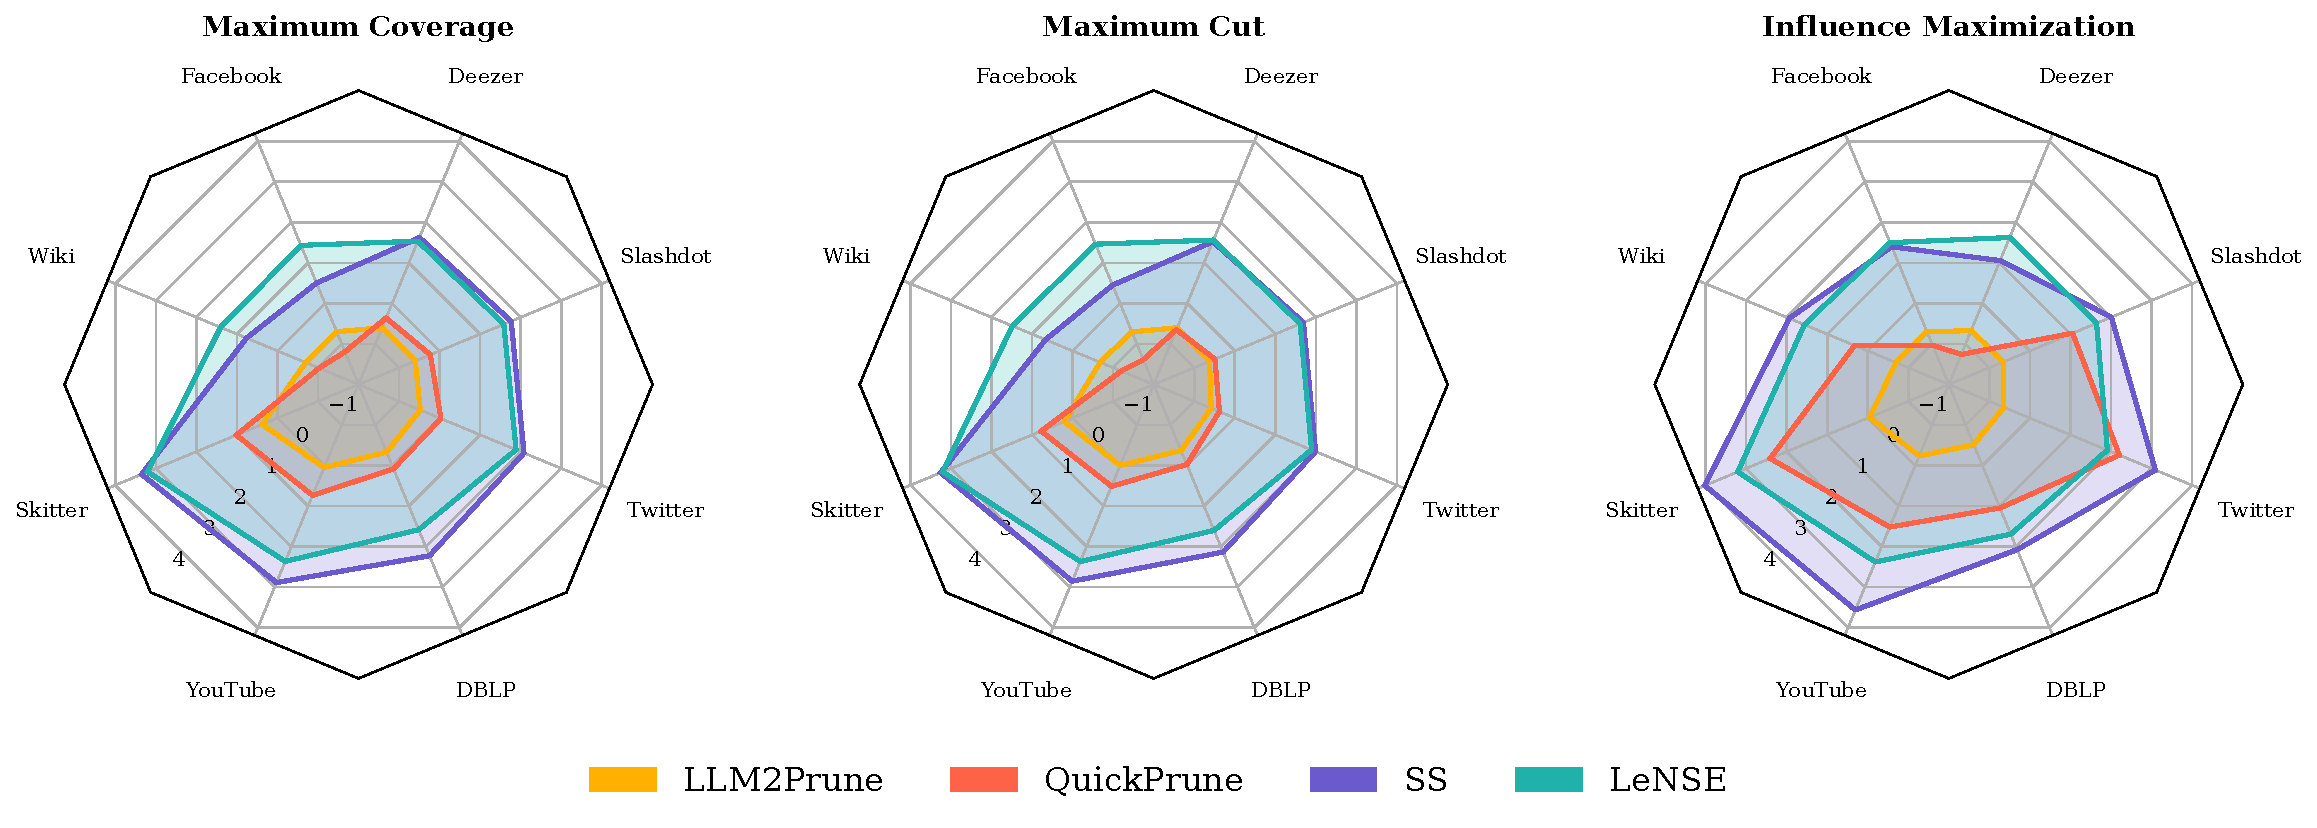
\includegraphics[width=0.9\linewidth]{figures/runtimes_radar.pdf}
    \caption{Runtime comparison (log scale) of pruning algorithms on Maximum Coverage, Maximum Cut, and Influence Maximization across eight datasets. }
    \label{fig:runtime}
\end{figure*}

\textbf{Applications.} We evaluate our algorithm on three problems: Maximum Coverage (MaxCover), Maximum Cut (MaxCut), and Influence Maximization (IM), under both size and knapsack constraints, following \cite{manchanda2020gcomb,ireland2022lense}. Detailed specifications of these applications are provided in Appendix \ref{appendix:applications}, along with the optimal features identified by our framework.

\textcolor{blue}{\textbf{Discovered Features.} A key strength of \llm is that it generates features that are not generic graph statistics but are grounded in the problem objective and constraints. For MaxCut, it discovers \emph{random cut expectation} (the expected marginal contribution of a node to the cut under a random partition), a non-trivial descriptor directly derived from the cut objective. For IM, it identifies \emph{average incoming activation probability} and \emph{outgoing activation probability sum}, which require reasoning about the independent cascade model and capture a node's susceptibility and direct influence spread respectively. Under the knapsack constraint, \llm automatically encodes the cost-benefit trade-off imposed by the constraint: for MaxCov it selects \emph{coverage per cost}, and for IM it selects \emph{degree-to-weight ratio} and \emph{in-out degree difference}, capturing both cost-efficiency and directional propagation asymmetry. These features would require significant domain expertise to design manually, yet \llm discovers them automatically from the task description alone. Full feature lists are provided in Appendix~\ref{appendix:applications}.}



\textbf{Baselines and Prior Methods.} We compare our algorithm with methods that accelerate heuristics by pruning the ground set rather than directly optimizing the objective function. Our evaluation includes the following classical and learning-based approaches: \textsc{QuickPrune}, \textsc{Submodular Sparsification (SS)}, GCOMB-P \citep{manchanda2020gcomb}, \textsc{LeNSE} \citep{ireland2022lense}, and \textsc{COMBHelper} \citep{tian2024combhelper}. Details of each baseline are provided in Appendix \ref{appendix:baselines}. For the general knapsack constraint, prior methods do not generalize, except for \qp, so we compare our algorithm only with \qp.

\textbf{Heuristics.} For both size and knapsack constraints, we follow \citep{pmlr-v258-nath25a}: for MaxCover and MaxCut, we use \textsc{Standard Greedy} \citep{nemhauser1978analysis}; for IM, we adopt IMM \citep{tang2015influence}; and under the knapsack constraint, we employ \cite{khuller1999budgeted} for IM and MaxCover, and \cite{pham2023linear} for MaxCut.

\textbf{Datasets.}  We evaluate our approach using real-world datasets from the Stanford Large Network Dataset Collection \citep{leskovec2016snap} for the CO problems on graphs, following the experimental setup of \cite{ireland2022lense}. A summary of all datasets used can be found in Appendix \ref{appendix:dataset}.

\textbf{Common Setup.} In all experiments, our algorithm and the baselines are trained to create a pruned ground set for CO problems with a budget of $k=100$, following \citet{ireland2022lense}. The downstream classifier, a two-layer GCN \citep{kipf2016semi}, operates on the LLM-proposed node-level features. To extract feature-importance vectors, we employ GNNExplainer \citep{kipf2016semi}. For each dataset, we adopt the train–test splits from \citet{ireland2022lense}. \textcolor{black}{We experiment with two LLMs, GPT-5-nano and LLaMA-3.3-70B-Instruct, to propose features, generate code, and summarize feedback. We report results using GPT-5-nano in the main paper. The two models achieve effectively comparable performance (as shown in Figure ~\ref{fig:models})}.




Since running beam search for features on each instance would be costly, and our main motivation is to reduce computation, we instead perform feature-space search for each problem using the Holme–Kim random graph model \citep{holme2002growing}. We select this model because it closely resembles large-scale social networks: it exhibits both the scale-free degree distribution and the high clustering coefficient that are empirically observed in real-world social graphs \citep{holme2002growing}. After identifying the feature set, we fine-tune the downstream classifier for each instance. Appendix~\ref{appendix:network} provides details on the network architecture, training and data generation hyperparameters, LLM settings, beam search, and baseline configurations.


\subsection{Evaluation on Size Constraint}

In this subsection, we first present our experiments under the size-constraint setting. Under this setting, each element in the ground set has a unit cost. All our baselines except \textsc{QuickPrune}, which works for both size and knapsack constraints, are designed specifically for the size constraint.

\textbf{Result Analysis.} From Table~\ref{tab:multi_problem_algos}, we observe that \llm performs competitively with classical methods such as \qp and SS. However, both approaches rely on sequential submodularity-based pruning, which is orders of magnitude slower than our method on large datasets such as YouTube and Skitter (as shown in Figure~\ref{fig:runtime}). In contrast, \llm achieves comparable or better performance without relying on hand-crafted features, demonstrating that learning-based pruning can be both effective and efficient.



Within the learning-based category, \llm outperforms prior methods in both combined metric and runtime. GCOMB-P and \textsc{COMBHelper} frequently underperform, while \textsc{LeNSE} is more stable but generally results in lower combined-metric values. Unlike other learning-based methods that depend on handcrafted features, \llm balances efficiency with strong performance, effectively narrowing the gap with classical methods.

\textbf{Runtime Analysis.} Figure~\ref{fig:runtime} reports the runtime of the four strongest algorithms across all applications. Classical methods are generally slower: SS is consistently the slowest, while \textsc{QuickPrune} is faster but scales poorly on large graphs. Among learning-based methods, \llm is orders of magnitude faster than \textsc{LeNSE} while maintaining higher solution quality, striking a strong balance between scalability and accuracy. Compared to other learning-based baselines, it also achieves the most consistent performance across applications. We report the \textcolor{blue}{absolute runtime analysis}, including an inference-time breakdown by component (see Appendix \ref{appendix:runtime}).

\textbf{Multi-budget Scores.} Following \cite{ireland2022lense}, we evaluate whether heuristics can also achieve close-to-optimal results for budgets lower than the one used to train the classifier. In our experiments, the classifier is trained to identify a pruned ground set for a budget of $100$. We then test whether the pruned ground set returned by the classifier can also be used for budgets below $100$. We observe that the ground set provided by \llm remains optimal for budgets lower than the training budget in nearly all instances. We report the multi-budget scores (see Appendix \ref{appendix:multibudget}). The results are qualitatively similar to our experiments under the knapsack constraint.

\subsection{Evaluation on Knapsack Constraint}

For the knapsack constraint, we adopt the cost model introduced by \citet{pmlr-v258-nath25a,pmlr-v108-yaroslavtsev20a}. Let $G = (V, E)$ be a graph with vertex set $V$ and edge set $E$. For each node $v \in V$, let $N(v) = \{ u \in V : (u,v) \in E \}$ denote its neighborhood. We define the cost of node $v$ as
$c(v) = \frac{\beta}{|V|}\bigl(|N(v)| - \alpha \bigr),$ where $\alpha = \tfrac{1}{20}$ is a fixed offset parameter, and $\beta > 0$ is a normalization factor chosen such that $c(v) \geq 1$ for all $v \in V$.  This cost model is more realistic for real-world graphs, where some nodes are inherently more expensive, for example, hubs in social networks or highly connected routers in communication networks. In contrast, a uniform cost unrealistically treats them as cheaply as sparsely connected nodes, which biases solutions toward hubs and can trivialize the optimization.

\textbf{Result Analysis.} As stated above, only \qp can be adopted to the knapsack constraint, so we compare our algorithm with \qp. We also compare it with another heuristic, TOP-k, following \cite{pmlr-v258-nath25a}. 

Figure~\ref{fig:knapsack} shows that \llm outperforms TOP-k across all applications, and outperforms \qp for MaxCov and IM, while slightly lagging behind in MaxCut. We highlight that, unlike other learning-based methods, \llm can easily adapt to the knapsack constraint by simply modifying the task description provided to the model.


 
\begin{figure}
    \centering
    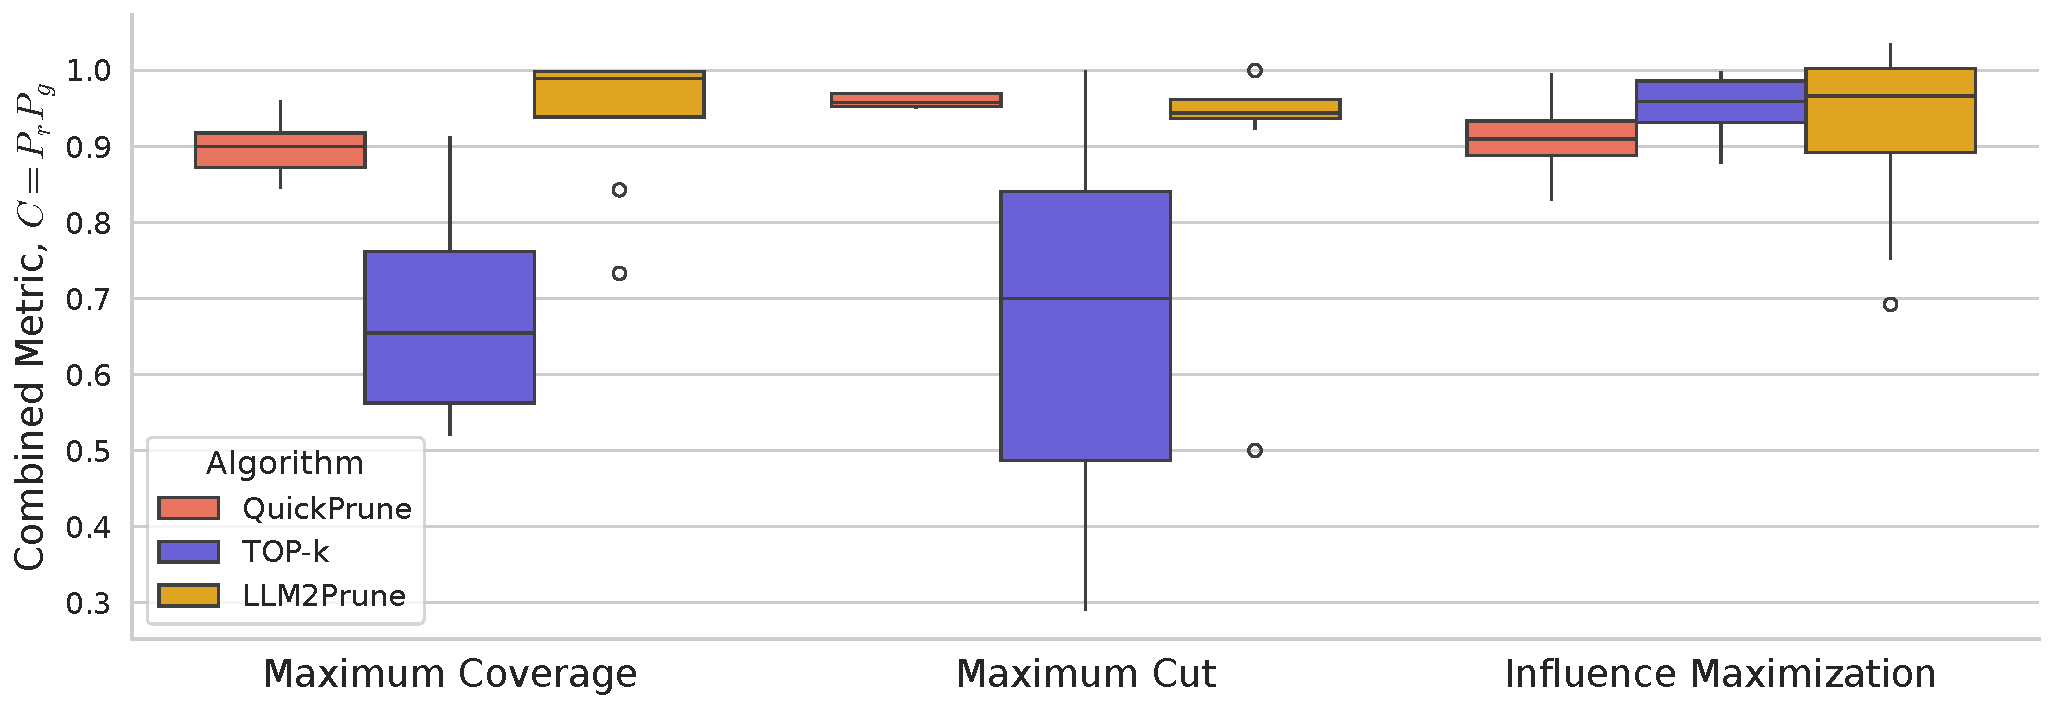
\includegraphics[width=\linewidth]{figures/algo_comparison_violin.pdf}
    \caption{Combined metric for \llm, \qp, and TOP-k under the knapsack constraint across MaxCov, MaxCut, and IM. \llm consistently outperforms TOP-k, matches or slightly exceeds \qp on MaxCov and IM, and is comparable to \qp on MaxCut.}
    \label{fig:knapsack}
\end{figure}





\textbf{Limitations and Future Directions.} A main limitation of \llm is the reliance on beam search, which is more computationally expensive than a simple feedback loop. As shown in Appendix~\ref{appendix:ablation}, simple feedback loops often fail to recover when early iterations contain reasoning errors, whereas beam search mitigates this issue by maintaining multiple candidate paths, at the cost of additional runtime. An important future direction is to reduce this overhead by leveraging reasoning tokens or similar mechanisms to improve the reliability of single-path feedback loops. Such approaches could capture richer intermediate reasoning without requiring multiple branches, thereby achieving the stability of beam search with significantly lower computational cost. \textcolor{blue}{Beyond computational cost, \llm is also sensitive to the choice of synthetic proxy used during feature discovery. When this proxy is structurally mismatched to the target graph family (for instance, Erd\H{o}s--R\'{e}nyi graphs, which have homogeneous degree distributions and lack clustering or community structure), the discovered features do not transfer well to real-world graphs. \llm therefore generalizes within a structural family but degrades under cross-family distribution shift.}


